\subsection{Help Requests}

Help request is a feature within the chatbot for admins/teacher where they can get an overview of which topic the chatbot currently has.
Under help request it possible for the admin to see which topics is troubling the students more. This is shown by a number in front of the topic which represent how many help request that topic has received by the students. This will help the teacher to know which topic is troubling the student so the teacher has the ability to go over that topic again.
Its also possible for the admin to look at all the classes that has been set up and see the students that are in those classes. Its also possible for the admin to help the students with their passwords and their login.
The admin also has the ability to add or remove students from the classes.

\begin{figure}[H]
    \centering
    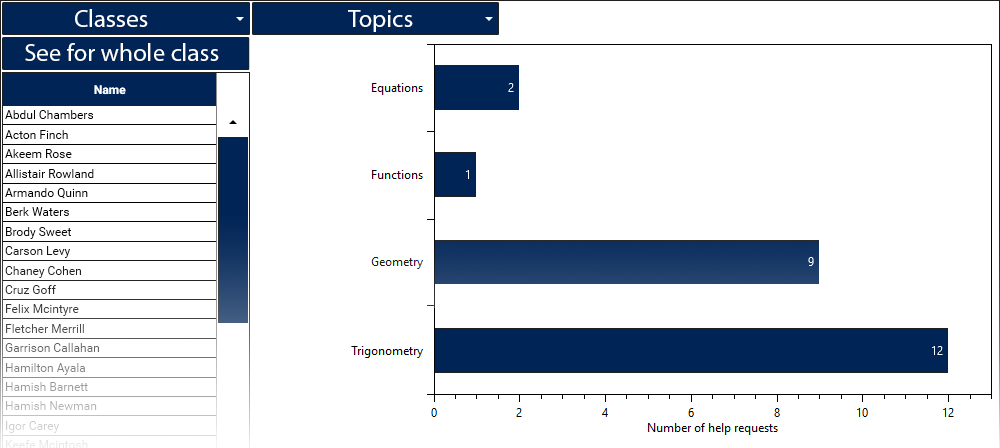
\includegraphics[width=0.6\textwidth]{figures/HelpRequest.png}
    \caption{Sketch of help request window}
    \label{fig:HelpRequest}
\end{figure}

\noindent
Figure \ref{fig:HelpRequest} above shows the admins view of help request. The admin has the option to click on the \enquote{All topics} to further more look into a specific topic to look more specific into what the is troubling the student under that topic.
Furthermore by clicking the \enquote{Classes} box a list will drop down with all the classes which then can be clicked on to view what that class is having trouble with.
Under the \enquote{Name} box all student in the selected class can be view and further more be looked more specific into.
